\documentclass[10pt]{beamer}
%\usecolortheme{beaver} 
\usetheme{Singapore}
\title{The Sudbury Neutrino Observatory}
\author{Yutong Du}
\institute[Berkeley]{Physics H190 Research Presentation}

\usepackage{chemformula}
\begin{document}
    \frame{\titlepage}

	\section{Overview}
    \begin{frame}
        \frametitle{What is SNO?}
		\begin{itemize}
			\item From SNO themselves: ``The goal of the observatory is to detect and study neutrinos emitted
				by the Sun and other celestial objects.'' 	
			\item A Heavy Water Cherenkov Detector
			\item Built in the Creighton Mine in Sudbury Ontario, 2km underground
			\item Largest underground cavity excavated at 2km depth
		\end{itemize}
            \end{frame}
	\section{Origins of SNO}
	\begin{frame}
		\frametitle{The Solar Neutrino Problem (SNP)}
		\begin{itemize}
			\item Previous neutrino observation data was only $\frac{1}{3}$ of what was predicted, but the 
				instrument was only sensitive to electron neutrinos $\nu_e$.
			\item \textbf{Hypothetical Solution:} The neutrinos change flavor over the course of their journey 
				from the Sun to the detector
				\item SNO's goal: verify this hypothesis
		\end{itemize}
	\end{frame}

	\begin{frame}
		\frametitle{Rough Timeline}
		\begin{itemize}
			\item 1985: Proposed solution to resolve the SNP via a Heavy-Water Cherenkov Detector
			\item 1989: US and Britain joins in on the project
			\item 1990: Construction begins
			\item November 1999: Construction completes, data collection (Phase I) begins. 
				\begin{itemize}
					\item May 2001: Phase II (NaCl $\rightarrow$ higher sensitivity)
					\item February 2004: Phase III (Neutral Current Detector)
				\end{itemize}
			\item November 2006: Data collection ends
			\item October 2015: Nobel Prize in Physics
		\end{itemize}
	\end{frame}

	\section{Instrumentation, Experiments}

	\begin{frame}
		\frametitle{Specs}

		\begin{itemize}
			\item Spherical Chamber 12 m across
			\item 9456 Hamamatsu R4108 photomulplier tubes
			\item 1000 tons of Heavy Water ($\ch{D2O}$)
			\item 7000 tons of ultra-pure normal water
		\end{itemize}


		\begin{center}
			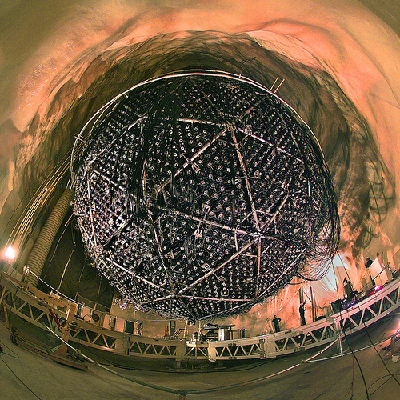
\includegraphics[scale=1]{outer_photo.jpeg} \phantom{aaaaaaa}
			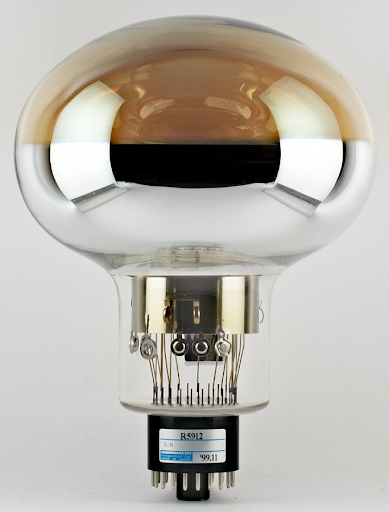
\includegraphics[scale=0.2]{photomultiplier.png}
		\end{center}

	\end{frame}

	\begin{frame}
		\frametitle{Detection Methods}
		\begin{block}{Neutral Current (NC)}
		\[ \nu_x + d \rightarrow p + n + \nu_x\]
		selects for all neutrinos equally
		\end{block}
		\begin{block}{Charged Current (CC)}
		\[ \nu_e + d \rightarrow p + p + e^-\]
		Only selects for electron neutrinos
		\end{block}
		\begin{block}{Elastic Scattering (ES)}
		\[ \nu_x + e^- \rightarrow \nu_x + e^-\]
		Selects for all neutrinos; $\nu_e$ selected 6x sensitivity
		\end{block} 
	\end{frame}

	\begin{frame}
		\frametitle{Feynman Diagrams}
		\begin{figure}
			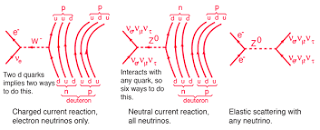
\includegraphics[scale=0.9]{reactions.png}
		\end{figure}
	\end{frame}

	\section{Accomplishments, Future}

	\begin{frame}
		\frametitle{Results}
	\begin{itemize}
		\item Total number of neutrinos detected matches theory $\rightarrow$ solves SNP
		\item Proves that Neutrinos have mass due to oscillations.
		\[ P_{\alpha \to \beta} = \sin^2(2\theta)\sin^2\left( \frac{\Delta m^2 L}{4E}\right)\]
		So $\Delta m > 0 \rightarrow$ neutrinos have mass!
		\item Data for solar mixing angle $\theta_{\text{sol}}$
	\end{itemize}
	\end{frame}

	\begin{frame}
		\frametitle{SNP Resolution}
		\begin{center}
			\begin{figure}
				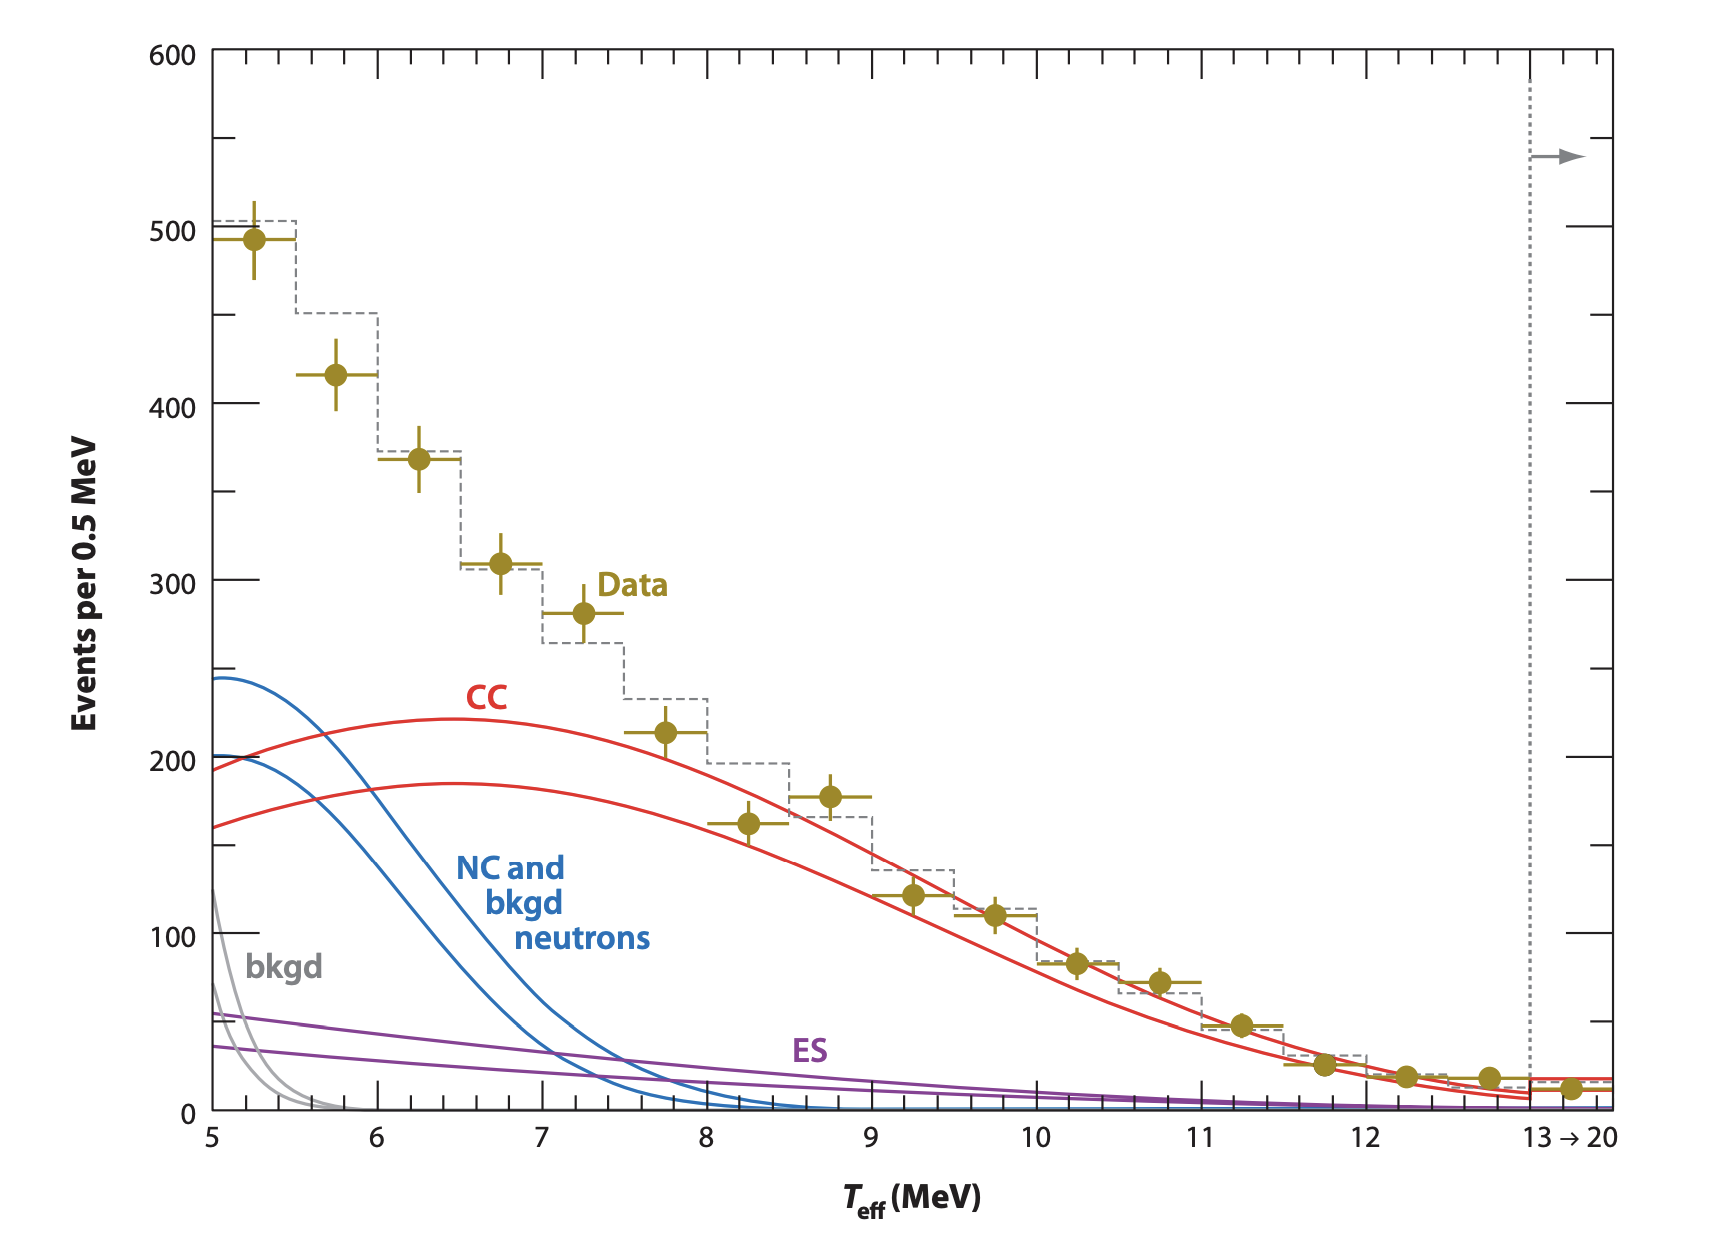
\includegraphics[scale=0.25]{plot2.png}
				\caption{Events vs. effective kinetic energy}
		\end{figure}
	\end{center}
	\end{frame}

	\begin{frame}
		\frametitle{Evidence of $\Delta m$}
		\begin{figure}
			\begin{center}
				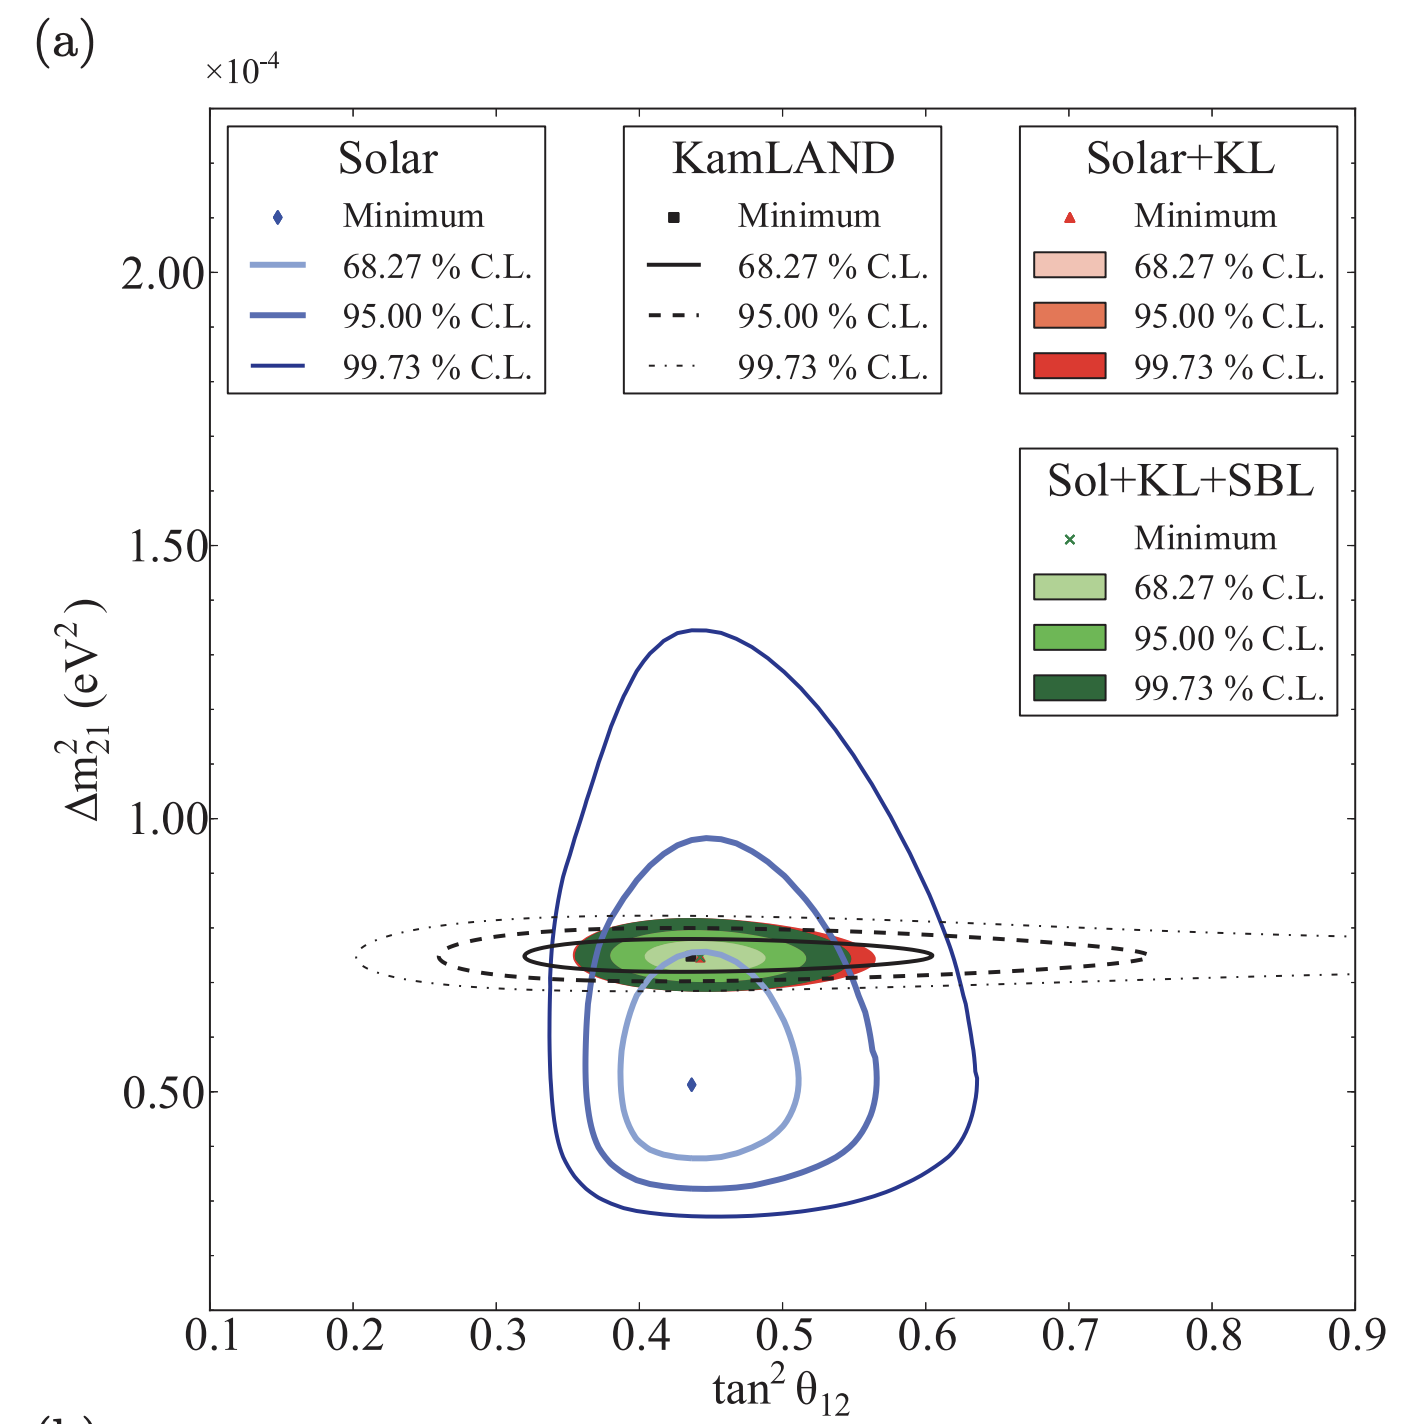
\includegraphics[scale=0.25]{oscillations.png}
			\end{center}
			\caption{Mixing angle $\tan^2\theta_{12}$ vs. $\Delta m_{21}^2$}
		\end{figure}
	\end{frame}

	\begin{frame}
		\frametitle{SNOLAB and Beyond}
		Since SNO, the mine was expanded to accomodate for more experiments, creating SNOLAB.
		\begin{itemize}
			\item SNO+: World's largest scintillator experiment
			\item SuperCDMS: Dark matter searches using Si and Ge crystals
			\item REPAIR: Effect of radiation on living organisms
		\end{itemize}

		\begin{center}
			\begin{figure}
				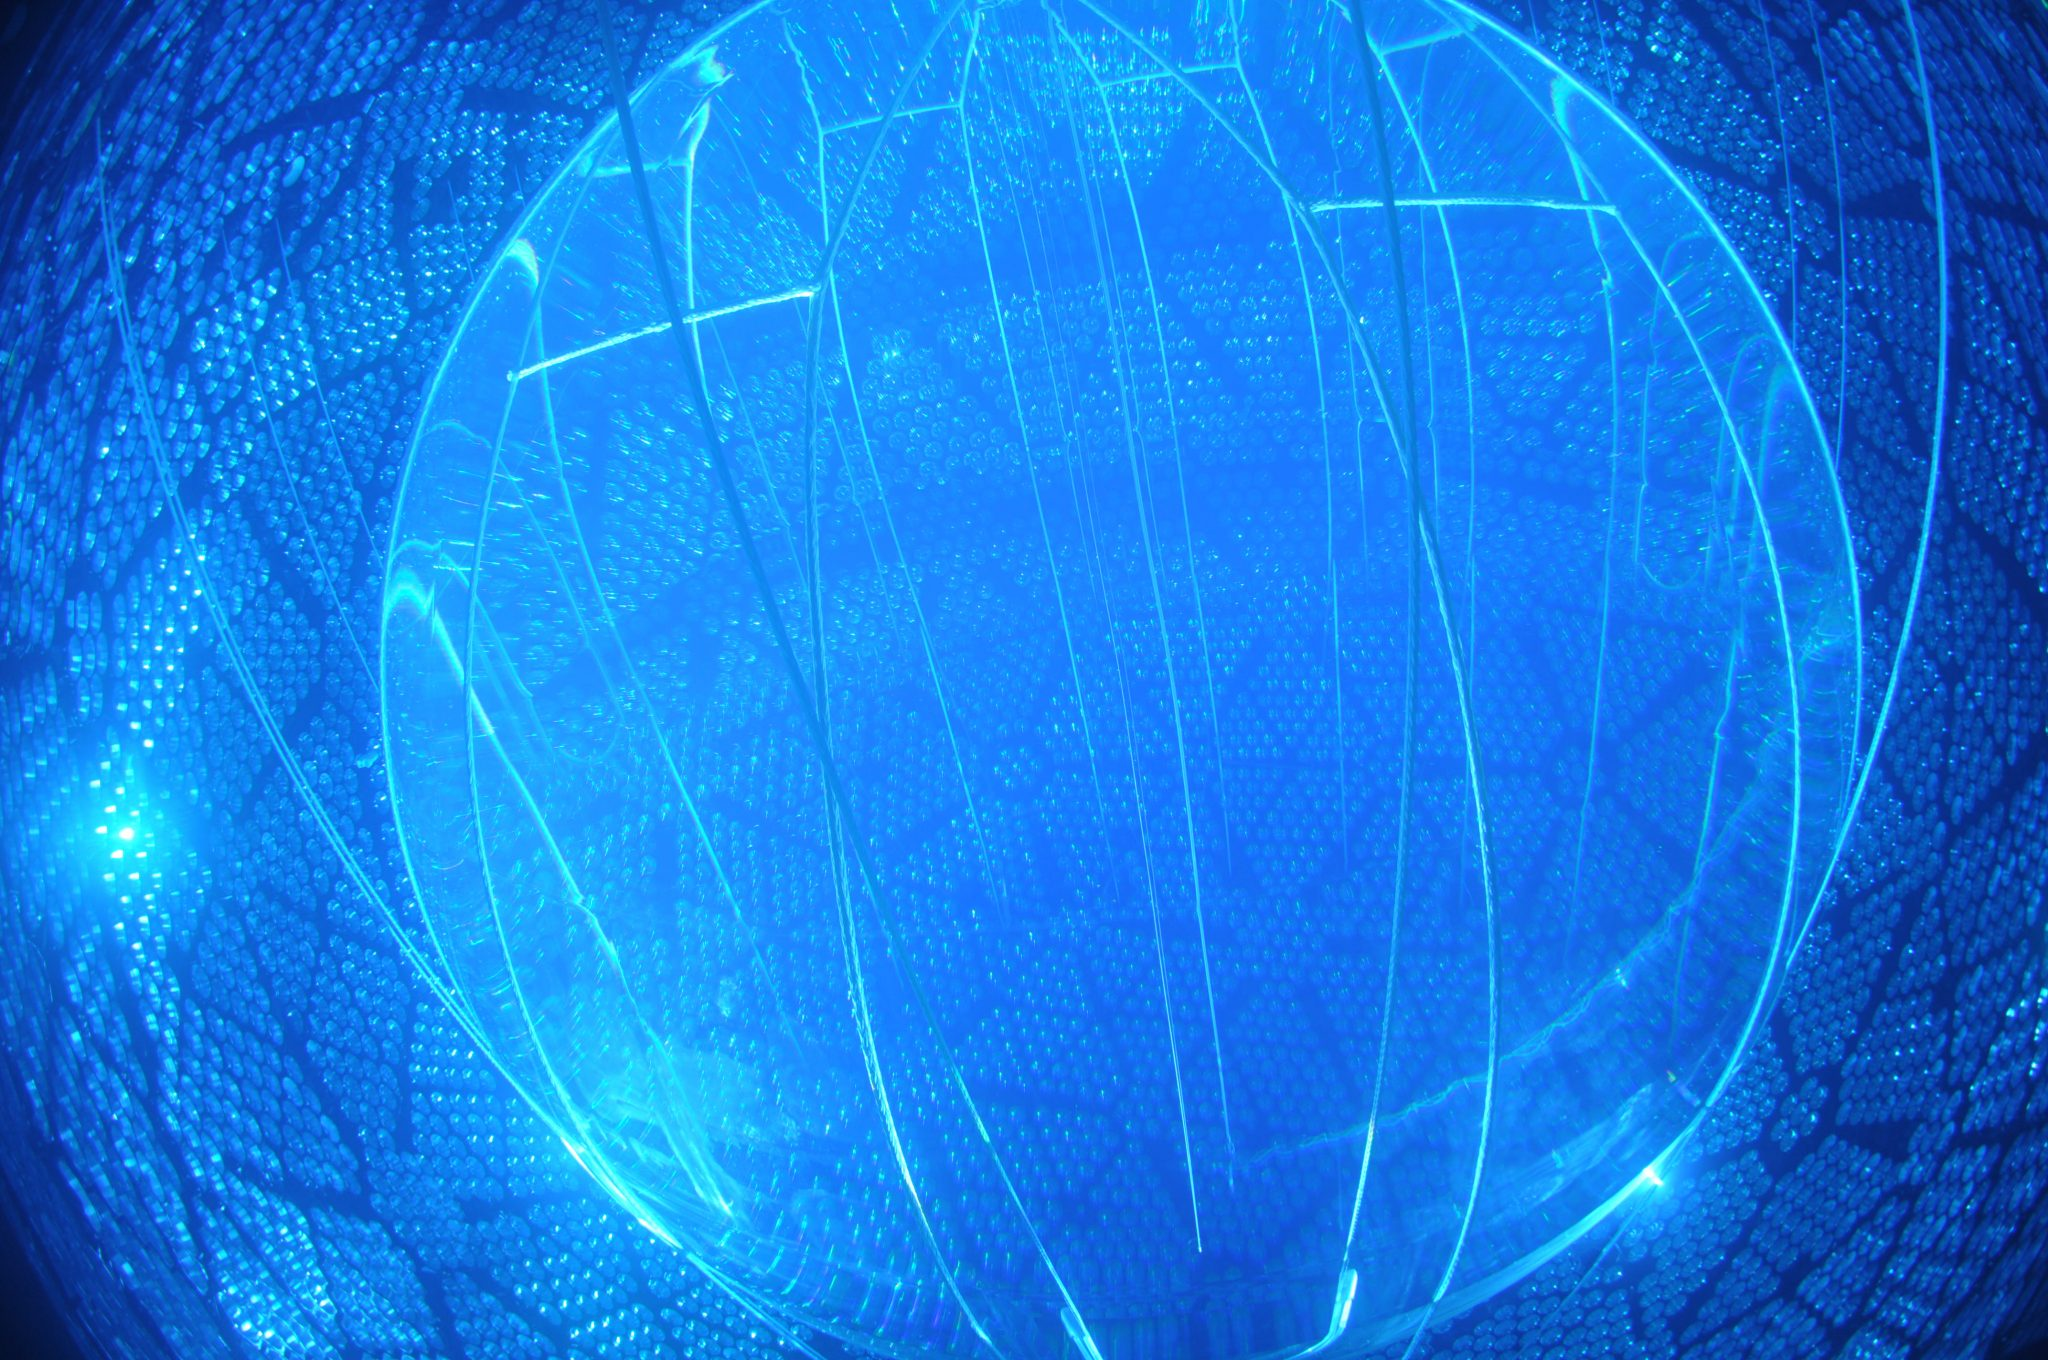
\includegraphics[scale=0.1]{sno+.jpeg}
				\caption{SNO+ detector}
			\end{figure}
		\end{center}
	\end{frame}
	\begin{frame}{References}
		\fontsize{10pt}{12pt}\selectfont
		\nocite{*}
		\bibliographystyle{unsrt} 
		\bibliography{references}
	\end{frame}
\end{document}


